
\documentclass[12pt,letterpaper]{report}
\usepackage{bbm}
\usepackage{dsfont}
\usepackage{multicol}
\usepackage{lipsum}
\usepackage{mwe}
\usepackage{graphicx}
\usepackage{epstopdf}
\epstopdfsetup{outdir=./}
\usepackage{subcaption}
\usepackage{geometry}
\usepackage{float}
\usepackage{amsmath,amssymb}
\usepackage{makecell}
\usepackage{lmodern}
\usepackage{mathtools}
\usepackage[thinc]{esdiff}
\usepackage{import}
\usepackage{braket}
\usepackage{enumerate}
\usepackage{listings}
\usepackage{biblatex}
\addbibresource{biblio.bib}
\usepackage{biblatex}

\DeclarePairedDelimiter{\ceil}{\lceil}{\rceil}

% Title Page
\title{ Dynamique moléculaire et simulation Monte-Carlo \\ 4: Introduction to Molecular Dynamics}
\author{Bruno Rodriguez Carrillo \\ EPFL}

\geometry{
	a4paper,
	total={185mm,260mm},
	left=15mm,
	top=15mm,
}

\begin{document}	
	\maketitle
	\section*{Time Evolution}
		
	\begin{enumerate}
		\item 
		Derive the form of $\mathbf{r}(t + \Delta t)$ in the velocity-Verlet (4.11). **Hint**: solve equation (4.10) for  $\mathbf{r}(t - \Delta t)$, and use equations (4.8) and (4.9).
		
		We have that equation (4.8) reads: 
		
		\begin{align}				
			\mathbf{r}(t + \Delta t) &= \mathbf{r}(t) + \mathbf{v}(t)\Delta t + \frac{1}{2}\mathbf{a}(t)\Delta t^2, \\
			\mathbf{r}(t - \Delta t) &= \mathbf{r}(t) - \mathbf{v}(t)\Delta t + \frac{1}{2}\mathbf{a}(t)\Delta t^2,
			\label{eq::4_8}
		\end{align}
		
		and equation (4.9) reads:
		\begin{align}				
		\mathbf{r}(t + \Delta t) = 2\mathbf{r}(t) - \mathbf{r}(t - \Delta t) + \mathbf{a}(t) \Delta t^2,
		\label{eq::4_9}
		\end{align}
	
		Solving equation (4.10) for  $\mathbf{r}(t - \Delta t)$, we have
		
		$$
			\mathbf{r}(t - \Delta t) =  \mathbf{r}(t + \Delta t) - 2 \mathbf{v}(t) \Delta t			
		$$
		
		And using (\ref{eq::4_9}), we have the result
		
		$$
		2 \mathbf{r}(t) + 2\mathbf{v}(t) \Delta t + \mathbf{a}(t) \Delta t^{2} = 2\mathbf{r}(t + \Delta t)
		\Rightarrow
		\mathbf{r}(t + \Delta t) =  \mathbf{r}(t) + \mathbf{v}(t) \Delta t + \dfrac{1}{2}\mathbf{a}(t) \Delta t^{2}
		$$		
		
		\item
		Derive the form of $\mathbf{v}(t + \Delta t)$ in the velocity-Verlet (4.11). **Hint**: recast equations (4.9) and (4.10) to a	timestep $\Delta t$ in the future, and use the result obtained  above.
			
		Now, recasting $\Delta t$ into the future and inserting the previous result into (4.9), we have
		
		$$
			\mathbf{r}(2t) = \mathbf{r}(t) + 2\mathbf{v}(t)\Delta t + \left( \mathbf{a}(t) + \mathbf{a}(t + \Delta t) \right) \Delta t^{2}
		$$
		
		Then from (4.10), we have
		
		$$
			\mathbf{r}(t + \Delta t) = \dfrac{ \mathbf{r}(2t) - \mathbf{r}(t) }{2 \Delta t}
			=
			\mathbf{v}(t) + \left( \mathbf{a}(t) + \dfrac{1}{2} \mathbf{a}(t + \Delta t) \right) \Delta t
		$$
		
		which is the desired result.
		
		\item
		Implement the velocity Verlet algorithm in the Toy MD program in `toy\_md.py`. Note, that the code only runs if you also implement the periodic boundary conditions function (see below).
		
		The implementation reads on the program `toy\_md.py` as: 
		
		\begin{figure}[H]
			\centering
			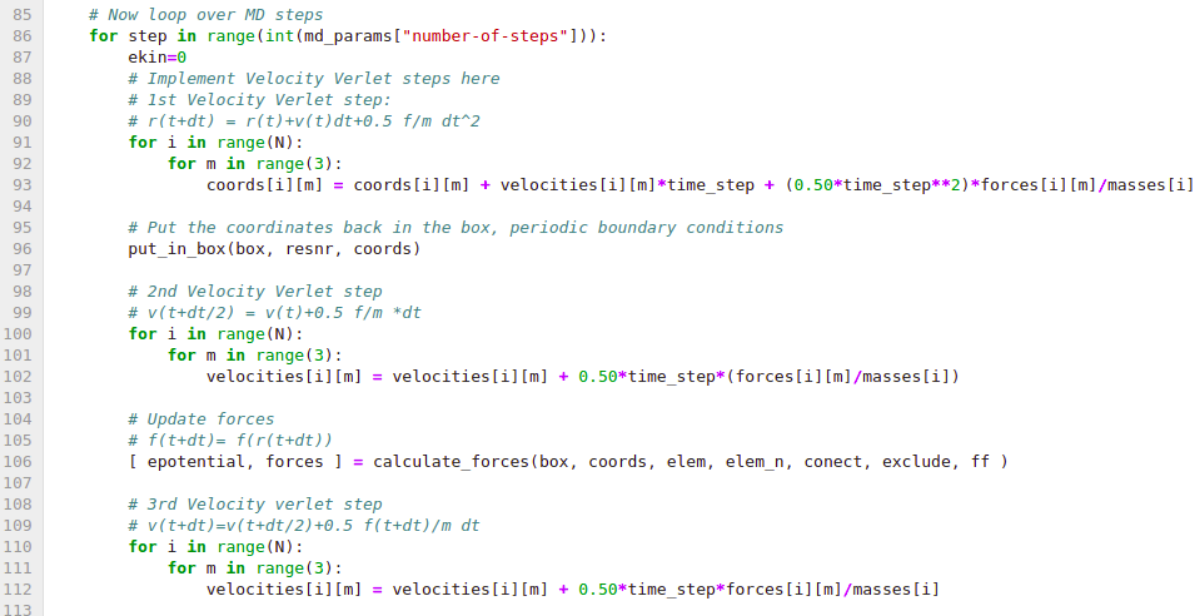
\includegraphics[width=0.6\linewidth]{velocityVerlet.png}		
			\caption{Velocity Verlet algorithm.}
			\label{fig::velocityVerlet}
		\end{figure} 
		
	\end{enumerate}

	
	\section*{Sampling Phase Space using Molecular Dynamics}	
	
	\begin{enumerate}
		\item 
		How does an MD program work? Describe schematically how one	performs a molecular dynamics simulation. Point out the main differences between your scheme and Monte Carlo methods. 
		
		From \cite{frenkel2001understanding}. First, we create a sample by selecting a model of N particles and then we solve the Newton's equations of motion for this system until the properties no longer change with time; this means that our system has reached equilibrium. 
		
		After the equilibrium phase is achieved, we start measuring the property or properties of interests during a certain time interval.
		
		To measure an observable $O$ during a MD simulation, we must express $O$ as a function of the positions and momenta of the particles in the system. 
		
		The MD program consists of: 
		\begin{enumerate}[a]
			\item 
			We read the parameters that specify the conditions of the run; that is initial values of temperature, number of particles, density, time-step size, position
			\item 
			We select te initial positions and velocities of the system			
			\item
			We compute the forces on all particles
			\item 		
			We integrate Newton's equations of motion. This point together with the previous one are repeated for the desired length of time
			\item 
			We compute the average of the measured quantities and the program stops			
		\end{enumerate}
		
		Based on \cite{thijssen_2007}: 
		
		Molecular dynamics consists basically of numerically integrating the Newton's equations of motion. It can therefore be viewed as a deterministic simulation of the system as it develops over a period of time. The system moves in phase space along its physical trajectory as determined by the equations of motion, whereas in the Monte Carlo method it follows a random walk. The great advantage of the MD method is that it not only provides a way to evaluate expectation values of static physical quantities; dynamical phenomena, such as transport of heat or charge, or relaxation of systems far from equilibrium can also be studied.
		
		\item
		Describe a possible implementation of periodic boundary conditions and provide an implementation in `toy\_md\_forces` to compute the distance of two particles taking into account the perodic boundary conditions in the `distance\_PBC` function (i.e a particle at the edge of the primary cell has a very short distance to the particle in the next cell). 
		With a box size of `[2,2,2]` and three points the elementwise distances between point `[0.5,0.5,0.5]` should be the same to the points `[-6.5,-6.5,-6.5]`, `[-2.5,-2.5,-2.5]`, `[1.5,1.5,1.5]`. The distance should be `[1,1,1]`. The distance to the identical point in an adjacent box (e.g [-1.5,-1.5,-1.5]) should be `[0, 0, 0]`.
		
		Taking 
		\begin{figure}[H]
			\centering
			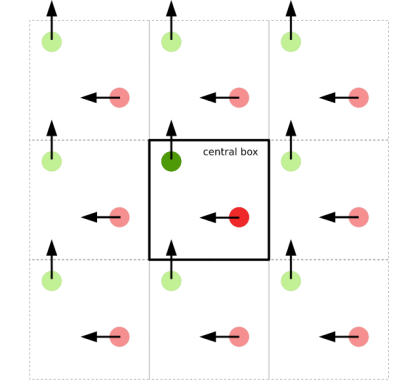
\includegraphics[width=0.25\linewidth]{pbc.png}		
			\caption{Periodic boundary conditions}
			\label{fig::pcb}
		\end{figure}  
		
		We want to compute the shortest distance for each component of our 3D system. This is done by element-wise computing the  distance between two particles and compare such a distance to the size of the box containing all particles. Let $d$ be the element-wise distance between two particles $X_{1}$ and $X_{2}$ and $l$ the box length. Then if $d > \dfrac{1}{2} l$, it means that we must bring the particle back inside the box, and then $d = d - l$; otherwise if $-2\cdot d > l$, then we update the distance by $d = d + l$ since the particle is contained in the box.
		
		As a result, we have the following implementation:
		
\begin{lstlisting}{language=Python}
def distance_pbc(box, x1, x2):
dx = np.zeros_like(box) # make an empty vector
for i in range(3):
	dx[i] = x1[i] - x2[i]
	if dx[i] > box[i]*0.50: 
	dx[i] = dx[i]- box[i] # bring the particle inside the box
	elif dx[i] <= -box[i]*0.50:
	dx[i] = dx[i] + box[i] #update distance                     
return dx
\end{lstlisting}
		
		\item		
		Why are most MD and MC simulations based on periodic systems?
		Explain the main purpose of periodic boundary conditions in these schemes.
		
		Taking what it is stated in \cite{thijssen_2007}, most computer simulations aim at describing a real-world problem. Unfortunately, the system size in such simulations is much smaller than those of experimental systems due to limited computational resources. The effects of considering smaller systems are felt through the presence of the boundary.
		The vast majority of molecular simulations, including Monte Carlo simulations, uses	periodic boundary conditions (PBC) as it is assumed that for these boundary conditions the behavior of the system is most similar to that of a system of the same size embedded in an infinite system. In fact, with periodic boundary
		conditions the system of interest is surrounded by similar systems with exactly	the same configuration of particles at any time. Besides, this implies that we can measure the property of interests in one box only. 
		
		We may think of PCB as those conditions that make possible simulate the behavior of an (possibly) infinite system by a finite one. The existence of PBC implies that any particle that leaves a simulation box enters the simulation box by the opposite side by which it leaves. This ensures that the number of particles is constant too.
			
		\item		
		**Bonus** What ensemble does the code in the ToyMD program sample in? Which of the quantities linear momentum $p$ and angular momentum $L$ are conserved when running with and without periodic boundary conditions?
		
		Once again, from \cite{thijssen_2007}, we have the following. We must be aware that under the minimum image convention the potential is no longer analytic, but discontinuities are irrelevant if the potential is significantly small beyond half the linear system size, as we implemented in the code. 
		
		Along the exact trajectory, energy is conserved as a result of the time-translation invariance of the Hamiltonian, but the energy of the numerical trajectory	will deviate from the exact value. Furthermore, as we have discussed, in molecular dynamics simulations the equations of motion for a set of particles are solved for forces depending on the relative positions of the particles only. In this case, energy and linear momentum $p$ are conserved; the particle number $N$ and system volume $V$ are conserved too since neither of these changes during the simulation. As a result, the time averages of physical quantities obtained by this type of simulation are equivalent to averages in the microcanonical (NVE) ensemble.
			
		On the other hand, the angular momentum $L$ is not conserved because of the periodic boundary conditions breaking the	spherical symmetry of the interactions.

	\end{enumerate}

	\newpage
	\printbibliography
	
%
%@article{giles_2015, title={Multilevel Monte Carlo methods}, volume={24}, DOI={10.1017/S096249291500001X}, journal={Acta Numerica}, publisher={Cambridge University Press}, author={Giles, Michael B.}, year={2015}, pages={259–328}}

\end{document}    